\documentclass[letterpaper]{article} % DO NOT CHANGE THIS
\usepackage[submission]{aaai2027}  % DO NOT CHANGE THIS
\usepackage[hyphens]{url}  % DO NOT CHANGE THIS
\usepackage{graphicx} % DO NOT CHANGE THIS
\urlstyle{rm} % DO NOT CHANGE THIS
\def\UrlFont{\rm}  % DO NOT CHANGE THIS
\usepackage{natbib}  % DO NOT CHANGE THIS AND DO NOT ADD ANY OPTIONS TO IT
\usepackage{caption} % DO NOT CHANGE THIS AND DO NOT ADD ANY OPTIONS TO IT
\frenchspacing  % DO NOT CHANGE THIS

\usepackage{booktabs}
\usepackage{amsmath}
\usepackage{amssymb}

\pdfinfo{
/TemplateVersion (2027.1)
}

\setcounter{secnumdepth}{0}

\title{Beyond Weight Geometry: Tracking On-Policy Distillation with Domain-Conditioned Functional Spectra}
\author{Anonymous Submission}
\affiliations{}

\begin{document}
\maketitle

\begin{abstract}
Weight geometry describes where parameters move, activation geometry describes which directions a model visits, and output evaluation records what the complete network produces. Missing is an observation layer for local computation that can be followed throughout training. We propose domain-conditioned functional spectra, which write the current weight of a linear module in whitened coordinates defined by an input domain's activation second moment. The singular spectrum then corresponds directly to module-output energy and admits an exact optimal low-rank output-error interpretation. We compare OPD, SFT, and offline distillation trajectories in two models, using sequence exposure, rollout refresh, and matched-support controls to tighten the interpretation. Strict dual-model common grids show that this functional coordinate retains trajectory and output-movement information not supplied by raw activation spectra or source-principal weight placement alone. OPD enters deeper cross-domain functional contraction in the shared early window, with continual current-student refresh organizing that path. Relative contraction also tracks unsigned movement in reasoning, formatting, answer, and termination regions, although similar functional paths can yield different readouts. The spectrum therefore provides a functional observation layer between bare weights and behavior, rather than a sufficient statistic for end-to-end performance.
\end{abstract}

\section{Introduction}

Post-training is not a single jump from an initial to a final model. Adjacent checkpoints can exhibit OOD degradation and recovery, abrupt changes in response length, termination failures, and strict-format drift. Endpoint comparisons discard these transients \citep{ren2026rethinking,jin2025rlheals}. The problem is especially pronounced in on-policy distillation (OPD): the current student generates rollouts and receives teacher-distribution supervision on those prefixes, so the training support co-evolves with the student \citep{agarwal2024opd,li2026rethinkingopd}.

Existing analyses observe three distinct levels. Weight geometry uses update norms, ranks, singular subspaces, and source-principal placement to describe parameter change \citep{shuttleworth2024lora,zhu2025path,yu2026dense,shen2026geometryopd}. Activation geometry uses effective rank, participation ratio, anisotropy, and CKA to describe which representational directions are visited \citep{liu2026collapse}. KL, NLL, and downstream tasks observe the output of the complete network. The first two omit either input visitation or the action of the weight map; the third collapses all layers and modules into final readout. None directly asks how the current weights use directions actually visited on a domain, or how that local computation evolves during training.

We address this gap with a domain-conditioned functional spectrum. For the weight $W_t$ of a linear module at checkpoint $t$ and a square root $S_{D,t}$ of its input-activation second moment on domain $D$, we analyze
\begin{equation}
A_{D,t}=W_tS_{D,t}.
\label{eq:intro-state}
\end{equation}
$A_{D,t}$ is not a post hoc concatenation of weight and activation features. It is the same weight map expressed in domain-conditioned whitened input coordinates. Its squared singular values are the eigenvalues of the module-output second moment, and truncating this spectrum minimizes expected layer-output error on $D$. The resulting functional rank asks how many directions are required to preserve the dominant output energy of the current module on that domain.

We turn this static local approximation space into a checkpoint-wise diagnostic and build a control chain around sequence support. OPD and off-KD share forward KL but use current-student and frozen-teacher sequences; an $\alpha=.5$ setting changes current-self exposure; frozenSelf0-KD fixes step-0 student rollouts and removes continuous refresh; and off-KD versus seqKD holds sequences fixed while changing soft to hard targets. Our contributions are:
\begin{itemize}
    \item A functional state variable with an exact layer-output error interpretation that, on strict dual-model common grids, retains trajectory information unavailable from raw activation spectra or source-principal weight placement alone.
    \item Cross-model evidence that OPD enters a deeper functional contraction regime in a shared early window. Exposure and frozen-self controls narrow this difference to the bundle induced by refreshing current support.
    \item Evidence that relative contraction tracks unsigned movement in reasoning, formatting, answer, and termination regions, while regional allocation, signed readout, and free generation remain model- and objective-dependent.
\end{itemize}

\section{Related Work}

\subsection{On-Policy Distillation and Training Trajectories}

Classical knowledge distillation matches soft teacher targets on fixed data \citep{hinton2015distilling}. GKD/OPD instead applies teacher feedback on states visited by the current student to reduce mismatch between training and inference support \citep{agarwal2024opd}. Subsequent work studies teacher--student gaps, cold start, support overlap, and feedback granularity \citep{li2026rethinkingopd,song2026surveyopd,yang2026oprd}. We do not propose another objective. We measure how sequence producer, support refresh, and target organize checkpoint-wise functional trajectories.

\subsection{Weight, Activation, and Functional Spaces}

Weight-space studies measure update scale, spectral concentration, principal-coordinate masks, source-principal projections, and singular-subspace rotation \citep{zhu2025path,jin2025rlheals,yu2026dense}. These quantities locate an update but do not vary with the input domain. Activation spectra and representation similarity describe how hidden states spread or reorganize, but not how the current weights amplify, suppress, or rotate those directions. Our $W_tS_{D,t}$ uses activations to define the input metric and then measures the complete current weight map in that metric. It therefore occupies a level between bare weights and final outputs rather than replacing either.

\subsection{Activation-Aware Low-Rank Approximation}

Bare-weight SVD minimizes Frobenius error in a Euclidean hidden-coordinate metric, treating frequently visited and nearly unvisited directions equally. Fisher-weighted SVD reweights the objective using an approximation to parameter sensitivity \citep{hsu2022fisherweighted}; ASVD and SVD-LLM use calibration activations to improve static weight decomposition \citep{yuan2024asvd,wang2025svdllm}. We retain the central activation-aware identity but change its role: instead of compressing a model once, we measure the current functional state at every checkpoint and domain. Relative to full-network Fisher, Jacobian, or Taylor diagnostics \citep{amari1998natural,martens2015kfac,saadi2025flex}, our construction is deliberately local. It is exact for a single-layer linear second-order problem and requires neither gradients nor a full-network approximation.

\section{Domain-Conditioned Functional Spectra}

\subsection{The Same Weight Map in Whitened Coordinates}

Fix a checkpoint, input domain, and linear module. For module input $h$, let
\begin{equation}
\Sigma_{D,t}=\mathbb E_{h\sim D}[hh^\top],
\qquad
S_{D,t}S_{D,t}^{\top}=\Sigma_{D,t}.
\label{eq:second-moment}
\end{equation}
If $\Sigma_{D,t}$ is full rank, set $z=S_{D,t}^{-1}h$; otherwise use $z=S_{D,t}^{\dagger}h$ on its support. Then
\begin{equation}
h=S_{D,t}z,\qquad \mathbb E[zz^\top]=I,\qquad
W_th=(W_tS_{D,t})z,
\label{eq:whitened-map}
\end{equation}
where $I$ is restricted to the support in the rank-deficient case. Thus $A_{D,t}=W_tS_{D,t}$ still represents $W_t$, but its input coordinates are whitened by the scales and correlations actually visited on $D$. A large bare-weight singular value need not generate a large domain output; the functional spectrum removes this coordinate-scale mismatch.

The representation also connects directly to layer output:
\begin{equation}
A_{D,t}A_{D,t}^{\top}
=W_t\Sigma_{D,t}W_t^\top
=\mathbb E[(W_th)(W_th)^\top].
\label{eq:output-energy}
\end{equation}
Hence $\sigma_i^2(A_{D,t})$ is the $i$th eigenvalue of the module-output second moment.
The bare-weight spectrum is precisely the special case $S=I$:
\begin{equation}
\mathbb E_{z:\,\mathbb E[zz^\top]=I}
\|(W_t-\widetilde W)z\|_2^2
=\|W_t-\widetilde W\|_F^2.
\end{equation}
It implicitly treats input directions as uncorrelated, unit-scale, and equally weighted;
$S_{D,t}$ replaces this isotropic metric by the one actually experienced on $D$. For
any candidate approximation $\widetilde W$,
\begin{equation}
\mathbb E\|W_th-\widetilde Wh\|_2^2
=\|(W_t-\widetilde W)S_{D,t}\|_F^2.
\label{eq:output-error}
\end{equation}
Writing $A_{D,t}=\sum_i\sigma_i u_iv_i^\top$, its top-$k$ truncation satisfies
\begin{equation}
\|A_{D,t}-A_{D,t}^{(k)}\|_F^2=\sum_{i>k}\sigma_i^2.
\end{equation}
Eckart--Young further lower-bounds the error of every rank-$k$ matrix by this tail energy
\citep{eckart1936approximation}. Together with Eq.~\eqref{eq:output-error}, discarding
the smaller functional singular directions exactly minimizes expected domain-conditioned
module-output error. Full proofs, the rank-deficient case, coordinate invariance, and
perturbation bounds are in Supplementary Secs.~A.1--A.5.

\subsection{Functional Rank and Trajectory Quantities}

For singular values $\sigma_1\ge\cdots\ge\sigma_q$ of $A_{D,t}$, define
\begin{equation}
r_\varepsilon(A_{D,t})
=\min\left\{r:
\frac{\sum_{i>r}\sigma_i^2}{\sum_i\sigma_i^2}\le\varepsilon
\right\}.
\label{eq:functional-rank}
\end{equation}
A smaller $r_\varepsilon$ means that dominant layer-output energy is concentrated in fewer functional modes. Main results use $\varepsilon=.05$; other thresholds, stable rank, and entropy effective rank audit threshold sensitivity.

The seven projections differ in shape and baseline functional rank; averaging raw
direction changes would let initially larger-rank modules dominate. To summarize the
reorganization of a typical projection relative to its own mode budget, the main
trajectory first normalizes within each module and then averages
\begin{equation}
\mathcal M_5=\{v,o,\mathrm{gate},\mathrm{up},\mathrm{down}\},
\end{equation}
giving
\begin{equation}
c_{\varepsilon,D,a,t}^{(5)}
=\frac{1}{5}\sum_{j\in\mathcal M_5}
\frac{r_{\varepsilon,D,a,0,j}-r_{\varepsilon,D,a,t,j}}
{r_{\varepsilon,D,a,0,j}}.
\label{eq:relative-contraction}
\end{equation}
Equal-5 is a relative summary across projection types, not an attribution of functional
energy. Query and key jointly determine attention routing, and their smaller baseline
functional ranks give a few direction changes high leverage. Their training-setting
orderings are also heterogeneous. We therefore report q/k and equal-7 separately.
Complete seven-module results appear in Supplementary Sec.~C.2.

\section{Experimental Design}

\subsection{Models, Training Settings, and Input Domains}

Experiments use Qwen3-4B-Base and Llama-3.2-3B students, both post-trained with rank-32
LoRA \citep{hu2022lora,qwen2025technical,meta2024llama32}. OPD uses current-student rollouts and dense
teacher distribution matching \citep{verl2025opd}; SFT uses external reference reasoning sequences and hard
next-token supervision. Because this pair changes producer, support, and target together,
we introduce controls by question. Off-KD retains teacher forward KL but replaces
current-student rollouts with frozen teacher sequences, testing sequence source. Qwen
$\alpha=.5$ changes current-student exposure under the same target. Llama frozenSelf0-KD
retains step-0 student-generated sequences but freezes them permanently, isolating
continual refresh. SeqKD shares the exact teacher sequences, order, steps, and LoRA
configuration of off-KD while replacing dense targets with hard next-token targets.

The four frozen domains have distinct roles. General uses WikiText slices as a
non-mathematical, non-instructional anchor \citep{merity2017pointer}. Held-out math uses Hendrycks MATH questions
deduplicated from training and MATH500 \citep{hendrycks2021math}. MMLU-Pro contains frozen questions and options
covering multidisciplinary knowledge and reasoning \citep{wang2024mmlupro}. IFEval contains only frozen
constraint prompts and probes format- and instruction-conditioned states \citep{zhou2023ifeval}. These texts
collect activations and are not behavioral scores. Qwen L18 and Llama L14 were selected
as architectural midpoints; samples, masks, deduplication, and layer repeats appear in
Supplementary Secs.~B.2 and C.3. Cross-setting comparisons use strict checkpoint
intersections; the shared early window is steps 20/40/80 and trajectory area ends at 320.

\subsection{Numerical and Statistical Protocol}

Functional spectra read serialized BF16 deployed merged checkpoints. Both tracks use BF16 forward passes, FP32 construction of $WS$, and FP64 symmetric eigendecomposition and SVD; Llama accumulates the Gram matrix in FP32 before FP64 factorization, whereas the Qwen audit track records Gram/whitening in FP64. We normalize within valid token windows per sample and then weight samples equally, preventing long texts from dominating. An independent numerical track yields Spearman $.9966$ and MAE $.00050$ for $r_{.05}$ on shared cells. Sample counts, masks, tie rules, dtype parity, and teacher top-32 retained-mass audits are in Supplementary Secs.~B.2--B.4.

Probes, domains, modules, and checkpoints are correlated measurements from one training
trajectory, not independent repetitions. Within-setting Spearman correlations describe
accumulated monotonic co-movement. Checkpoint demeaning subtracts the four-setting mean
within each model--domain--checkpoint and tests cross-setting information at a fixed
training stage. Held-out models leave out complete checkpoint groups; standardization
and ridge selection use only training folds.

\subsection{Regional Outputs and Comparison Coordinates}

We teacher-force fixed reference sequences and compute full-vocabulary
$D_{\mathrm{KL}}(p_0\Vert p_t)$ from base to checkpoint. MMLU-Pro is split into prompt
$P$, pre-label format tokens $F$, the correct answer-choice label $A$, and termination
$T$. MATH500 is split into prompt $P$, reference reasoning before the final box $C$, a
token-clean complete boxed-answer span $B$, and termination $T$. Main KL regions are
$F/A/T$ and $C/B/T$; values are averaged within each sample region and then
macro-averaged. Signed NLL retains whether reference-token likelihood improves or worsens.
Full masks, token boundaries, and whole-reference-stream sensitivity are in Supplementary
Secs.~B.2 and D.1.

Comparison coordinates cover activations, update placement, and weight subspaces. The
activation representative is entropy effective rank \citep{liu2026collapse},
\begin{equation}
\mathrm{ER}=\exp\!\left(-\sum_iq_i\log q_i\right),\qquad
q_i=\lambda_i/\sum_j\lambda_j.
\end{equation}
TPNT measures enrichment of update coordinates in a source rank-$k$ principal mask
relative to an equal-density null \citep{yu2026dense,zhu2025path}. PABS averages principal-angle cosines between source
and checkpoint top-$k$ left/right singular subspaces; values near one indicate little
rotation \citep{jin2025rlheals}. The full activation suite $A$ also contains PR, top-1/8/32 shares,
raw/centered anisotropy, and step-0 CKA. A strong weight-only baseline \citep{yu2026dense} is
\begin{equation}
p_k=\frac{\|U_k^\top\Delta W V_k\|_F^2}{\|\Delta W\|_F^2},
\qquad k\in\{4,8,16,32\},
\label{eq:pk}
\end{equation}
where $U_k,V_k$ are top-$k$ source-weight singular subspaces and $\Delta W$ is deployed
merged checkpoint minus base. NSS and the remaining native metrics are detailed in
Supplementary Sec.~B.4. Comparisons use shared cells, the same module set, and identical
checkpoint-held-out folds.

\section{Results}

\begin{figure*}[!t]
\centering
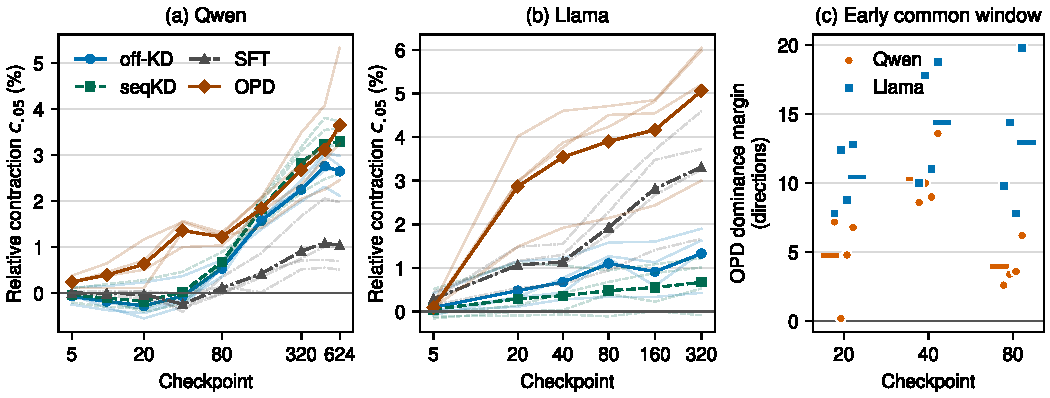
\includegraphics[width=\textwidth]{figures/fig1_main_trajectories.pdf}
\caption{Activation, weight, and functional trajectories. Rows show Qwen and Llama;
columns show activation ER, TPNT excess lift above its null, PABS drift
$10^4(1-\mathrm{PABS})$, and equal-5 relative functional contraction. Column scales have
different units and raw magnitudes are not comparable. Lines connect observed checkpoints
only. Functional contraction exposes training-setting separation not jointly reproduced
by the preceding coordinates.}
\label{fig:main}
\end{figure*}

\begin{table*}[!t]
\centering
\small
\setlength{\tabcolsep}{5pt}
\begin{tabular}{lccc}
\toprule
Model & Activation suite $A$ & Functional $C_5$ & Weight $P_{k,5}$ \\
\midrule
Llama & .556 & \textbf{.743} & .688 \\
Qwen & .595 & \textbf{.708} & .521 \\
\bottomrule
\end{tabular}
\caption{OPD identification on strict common grids (checkpoint-held-out AUC). Each model
uses 64 common states, identical equal-5 modules, and identical folds. $A$ is the
eight-feature activation suite containing ER, PR, top-1/8/32 shares, raw/centered
anisotropy, and step-0 CKA; it is not the single ER trajectory in Figure~\ref{fig:main}.}
\label{tab:identification}
\end{table*}

\begin{table*}[!t]
\centering
\small
\setlength{\tabcolsep}{4pt}
\begin{tabular}{lrrrrr}
\toprule
Model & $M_{\min}^{\mathrm{early}}$ & OPD NCD & SFT NCD & off-KD NCD & seqKD NCD \\
\midrule
Qwen & .200 & \textbf{50.423} & 9.554 & 31.017 & 37.793 \\
Llama & 7.800 & \textbf{77.594} & 39.683 & 17.518 & 11.093 \\
\bottomrule
\end{tabular}
\caption{Shared early ordering and full-trajectory contraction dose.
$M_{\min}^{\mathrm{early}}$ is the minimum continuous OPD margin over four core domains
and shared early checkpoints (directions); positivity excludes a reversal on this grid.
NCD integrates depth and duration through $T=320$ in directions$\times$log-step. The
two columns have different units and are not numerically comparable.}
\label{tab:ncd}
\end{table*}

\begin{figure*}[!t]
\centering
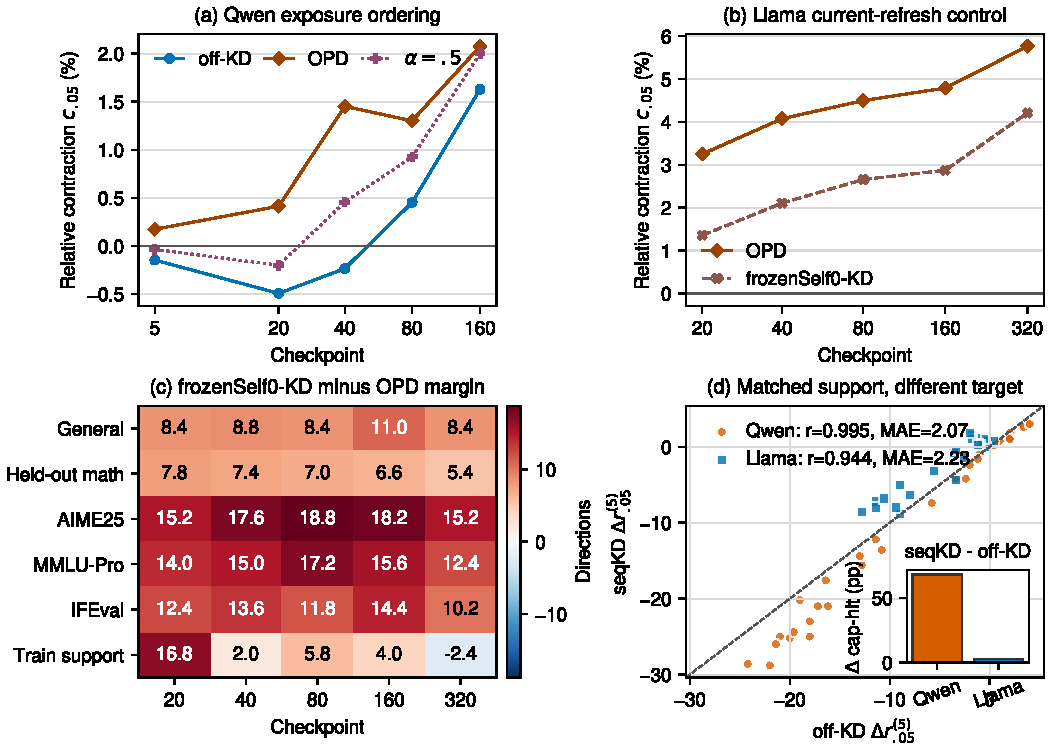
\includegraphics[width=\textwidth]{figures/fig2_support_controls.pdf}
\caption{Sequence-exposure and refresh controls. (a) Ordered Qwen $\alpha=.5$ movement
relative to off-KD and OPD. (b) Mean absolute trajectories of Llama OPD and
frozenSelf0-KD over five fixed external domains. (c) Corresponding paired margins;
positive values indicate deeper contraction under continuously refreshed OPD, and the
thick black line is the external-domain mean. Math, AIME, MMLU, and Mean denote held-out
math, AIME25, MMLU-Pro, and the five-domain mean.}
\label{fig:controls}
\end{figure*}

\begin{table*}[!t]
\centering
\small
\setlength{\tabcolsep}{2.7pt}
\textbf{A. Per-domain equal-5 path agreement, off-KD vs. seqKD
(Pearson $r$/MAE directions)}\\[2pt]
\begin{tabular}{lccccc}
\toprule
Model & General & Math & MMLU-Pro & IFEval & Pooled \\
\midrule
Qwen & .995/1.13 & .996/2.67 & .998/2.18 & .999/2.29 & .995/2.07 \\
Llama & -.771/2.53 & .971/1.73 & .968/2.23 & .824/2.40 & .944/2.23 \\
\bottomrule
\end{tabular}

\vspace{4pt}
\textbf{B. Endpoint behavior for matched-support settings (\%)}\\[2pt]
\begin{tabular}{llrrrrrrr}
\toprule
Model & Setting & \multicolumn{2}{c}{MATH500} & \multicolumn{3}{c}{MMLU-Pro} & \multicolumn{2}{c}{IFEval} \\
\cmidrule(lr){3-4}\cmidrule(lr){5-7}\cmidrule(lr){8-9}
 & & Acc. & Cap & Strict & Flex. & Extract & Prompt & Instr. \\
\midrule
Qwen & off-KD & 79.4 & 4.8 & 35.4 & 57.1 & 47.3 & 23.1 & 36.5 \\
 & seqKD & 72.4 & 73.0 & 30.6 & 58.1 & 54.1 & 24.4 & 39.3 \\
Llama & off-KD & 8.2 & 91.8 & 14.2 & 16.4 & 50.3 & 19.6 & 33.2 \\
 & seqKD & 10.2 & 94.6 & 13.1 & 15.4 & 51.6 & 19.2 & 31.5 \\
\bottomrule
\end{tabular}
\caption{Matched-support functional paths and behavioral readout. A uses matched nonzero
checkpoints; MAE is the checkpoint-wise direction difference. B uses Qwen step 624 and
Llama step 320. Cap denotes generation-cap hit, Extract extraction failure, and
Prompt/Instr. IFEval prompt/instruction strict.}
\label{tab:support-readout}
\end{table*}

\begin{figure*}[!t]
\centering
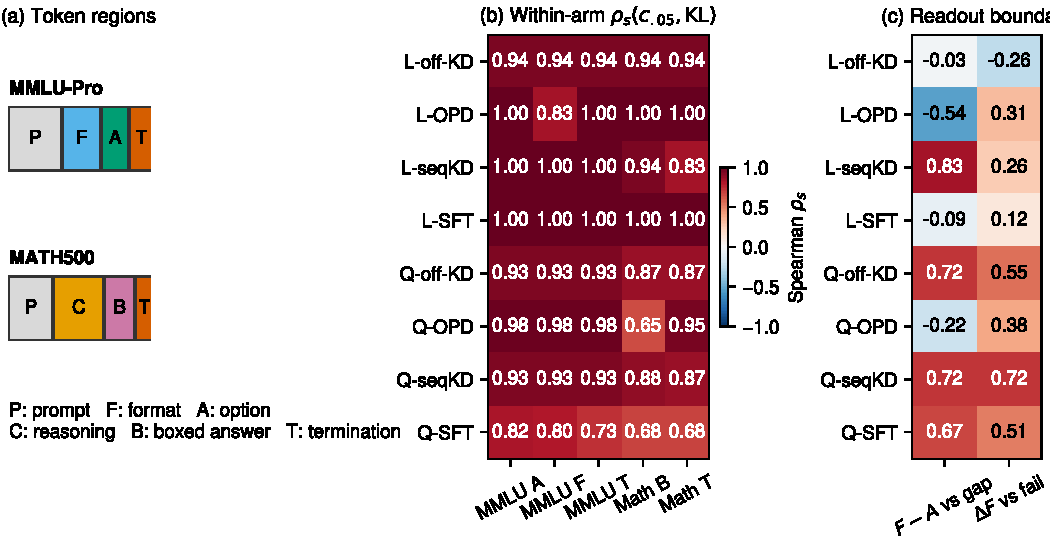
\includegraphics[width=\textwidth]{figures/fig3_regional_output.pdf}
\caption{Regional output relationships. (a) Within-model, within-setting Spearman
correlations between equal-5 functional contraction and regional full-vocabulary KL.
MMLU-Pro columns are format ($F$), correct answer-choice label ($A$), and termination
($T$); MATH500 columns are reasoning ($C$), boxed answer ($B$), and termination ($T$).
(b) MMLU-Pro correlations of the format--answer signed-NLL contrast with the
strict--flexible gap and of format NLL with extraction failure. L and Q denote Llama and
Qwen; each cell prints its correlation.}
\label{fig:regional}
\end{figure*}

\begin{table*}[!t]
\centering
\small
\setlength{\tabcolsep}{4pt}
\begin{tabular}{llcc}
\toprule
Model/domain & Regions & Held-out $R^2$: $C_5$ & Best $P_{k,5}$ \\
\midrule
Llama / MMLU-Pro & $A/F/T$ & \textbf{.869/.932/.468} & .743/.788/.459 \\
Llama / MATH500 & $B/T$ & .561/\textbf{.812} & \textbf{.615}/.647 \\
Qwen / MMLU-Pro & $A/F/T$ & \textbf{.426/.577/.596} & .243/.318/.443 \\
Qwen / MATH500 & $B/T$ & \textbf{.227}/.604 & .167/\textbf{.718} \\
\bottomrule
\end{tabular}
\caption{Out-of-fold prediction of regional full-vocabulary KL. $C_5$ and $P_{k,5}$
use the same five modules, states, and checkpoint-held-out folds. Values follow the
region order; bold marks the higher per-region $R^2$. The later Math $C$ audit is
reported within trajectories and after checkpoint demeaning, but is not included in
this matched held-out table.}
\label{tab:regional-prediction}
\end{table*}


\subsection{Functional Spectra Add Information Beyond Activation and Weight Coordinates}

Figure~\ref{fig:main} places four observables on the same training settings and checkpoints.
ER measures the spectral dimension of activation covariance; TPNT measures enrichment of
update coordinates in a source-principal mask; PABS measures rotation of dominant weight
subspaces; the functional spectrum measures output modes formed by the current weight on
directions actually visited by a domain. Their vertical scales are incomparable, but
their trajectory structure can be compared.

Activation trajectories do not reproduce the functional separation. Across several
external Llama domains, ER changes by less than $.003$ at OPD@160 and step-0 CKA remains
approximately $.9997$--$1.0000$, while $r_{.05}$ at the same locations has fallen by
roughly 14--26 directions. TPNT shows local enrichment above a spectrum-matched null at
some checkpoints but no stable cross-model OPD-specific path. PABS remains close to one,
with small NSS, indicating that these LoRA trajectories evolve largely within a nearly
fixed dominant weight basis. Equal-5 functional contraction, in contrast, clearly
separates the training settings in the last column of Figure~\ref{fig:main}. This
difference comes from the joint action of $W_t$ and the domain input metric, not merely
from adding more features. Native metrics, nulls, and layer results are in Supplementary
Secs.~B.4 and C.3.

We then leave out checkpoint groups on 64 strictly common states per model.
Table~\ref{tab:identification} compares the complete activation suite $A$, functional
contraction $C_5$, and source-principal block $P_{k,5}$. $C_5$ provides stronger OPD
ranking in both models and exceeds raw activations on all three output targets under the
same protocol. Strict $p_k$ retains a local Qwen absolute-NLL advantage, so functional
state and update placement remain task-dependent complements rather than a universal
dominance relation (Supplementary Sec.~D.3).

\subsection{OPD Dominates Shared Early Functional Contraction}

The last column of Figure~\ref{fig:main} shows deeper early OPD contraction in both
models. To test whether domain averaging hides a reversal, define the margin over the
nearest offline setting:
\begin{equation}
M_{m,D,t}
=\min_{b\in\{\mathrm{SFT,offKD,seqKD}\}}\Delta r_{m,b,D,t}^{(5)}
-\Delta r_{m,\mathrm{OPD},D,t}^{(5)}.
\end{equation}
$M>0$ means that OPD contracts more than every offline setting. At
$\varepsilon=.05$, the minimum margin across four core domains and steps 20/40/80 is
positive for both models; complete domain curves are in Supplementary Sec.~C.1. We also
integrate below-base contraction in $\tau=\log(1+t)$ through $T=320$ to obtain negative
contraction dose (NCD). Table~\ref{tab:ncd} keeps early ordering and full-trajectory dose
separate; OPD has the largest NCD in both models.

Four thresholds, continuous spectra, centered covariance, and layer audits preserve this
conclusion. Module audits show that the OPD-deepest ordering is more stable in
value/output and MLP projections, whereas q/k are heterogeneous; this is not an
attribution of contraction energy to five modules. Complete equal-7, layer, and module
results are in Supplementary Secs.~C.2--C.3.

\subsection{Exposure and Refresh Organize Trajectories, Not Readout}

Under the same forward-KL target, Qwen $\alpha=.5$ moves in an ordered direction from
off-KD toward OPD without forming an exact one-dimensional interpolation
(Figure~\ref{fig:controls}a). Llama frozenSelf0-KD instead removes only continual refresh
of current-student rollouts. OPD's contraction advantage persists at all later checkpoints
on five fixed external domains (Figures~\ref{fig:controls}b--c), making the
current-support refresh bundle the more direct organizer. Because refresh jointly changes
rollout length, EOS, repetition, and style, this control identifies the aggregate refresh
bundle rather than a pure freshness effect.

Off-KD and seqKD use identical teacher sequences, order, steps, and LoRA configuration,
changing only the target. Table~\ref{tab:support-readout}A shows highly aligned paths
across all four Qwen domains; Llama mode budgets remain close, although temporal
co-movement is heterogeneous on General. Readout is not locked by these paths. Qwen
seqKD has a much higher endpoint MATH500 cap-hit rate, with accuracy and formatting
changes, while Llama does not reproduce a divergence of comparable size
(Table~\ref{tab:support-readout}B). Matched sequence support can organize a similar
functional-mode budget while target distribution changes its realization.

\subsection{Relative Contraction Tracks Regional Unsigned Movement}

Figure~\ref{fig:regional}a compares $c_{.05}^{(5)}$ with regional KL within each training
setting. Formatting, answer, and termination on MMLU, and reasoning, boxed answer, and
termination on MATH, mostly move with functional contraction. Math CoT is positive in
all four settings of both models. To fix training stage, we subtract the contemporaneous
four-setting mean within each model--domain--checkpoint. Math $\mathrm{KL}_C$ remains
correlated at $.875/.573$ in Llama/Qwen, compared with $.902/.440$ for
$\mathrm{KL}_B$; the regional contrast $\mathrm{KL}_B-\mathrm{KL}_C$ is
$-.209/-.183$. Functional contraction therefore tracks how far each region moves but
does not determine whether movement is allocated primarily to reasoning or final answer.

Table~\ref{tab:regional-prediction} compares $C_5$ with the strong weight baseline
$P_{k,5}$ on the originally frozen actual-KL regions. Functional contraction has higher
held-out $R^2$ in most regions, with explicit exceptions for Llama Math boxed answer and
Qwen Math termination. This matched comparison does not yet include the later Math $C$
audit, so we do not fold the new region into the old win summary. Across signed and
absolute targets the average gap narrows, and the unsigned relation also persists when
the full fixed reference completion is merged into one region (Supplementary
Secs.~D.1--D.3).

\subsection{Signed Readout and Behavior Are Model-Dependent}

KL measures movement magnitude; signed NLL asks whether reference tokens become easier
or harder. MMLU-Pro $\Delta\mathrm{NLL}_{F-A}$ contrasts format and answer, while MATH
$\Delta\mathrm{NLL}_{B-C}$ contrasts boxed answer and preceding reasoning. Their
relationships to strict--flexible gaps or extraction failure change sign across models
and settings (Figure~\ref{fig:regional}b). For example, $F-A$ is positively associated
with the format gap in Qwen off-KD/seqKD but negatively associated in Qwen OPD and Llama
OPD. Functional mode count, regional allocation, reference-token valence, and free
generation are related but non-interchangeable levels.

This boundary agrees with matched support. Functional spectra describe how sequence
support organizes local mode budgets and how far output distributions move, but one rank
cannot determine whether that movement improves or harms a task. Qwen adapter zeroing
and answer-position probability-mass audits further support a formatting/readout-channel
account, but remain model-specific evidence (Supplementary Sec.~D.5).


\section{Discussion}

The value of a domain-conditioned functional spectrum is not to replace bare weights or output evaluation, but to provide a mode-separating intermediate observation. Bare-weight coordinates show where an update enters the source parameter structure, and behavioral evaluation determines whether the complete model performs a task. $W_tS_{D,t}$ instead places the current weight in coordinates actually visited on a domain, giving each singular mode a direct layer-output energy meaning. It can therefore distinguish cases with similar parameter placement but different functional budgets, and cases with similar functional budgets but different readouts.

Functional contraction is not synonymous with capability deletion. It means that
dominant module-output energy is concentrated into fewer modes. Those modes may be
efficient or may route probability mass into unsuitable reasoning, formatting, or
termination channels. Regional KL further shows that mode count, regional allocation,
readout valence, and sequence-level task realization cannot be collapsed onto one axis.

\section{Limitations}

Several limitations remain. First, the theoretical characterization is exact only for the module-local, layer-linear second-order output error of an individual module, and does not account for cross-layer nonlinearities, residual pathways, or final token readout. Second, the observed relationships between the proposed functional observable and downstream behavior are empirical associations rather than end-to-end causal attributions; the intervening mechanisms connecting local functional geometry to final model behavior therefore remain unidentified. Third, the current experiments consider only a limited set of exposure coefficients ($\alpha$), precluding a densely controlled characterization of the exposure-response relationship and a direct assessment of whether the reported ordering varies continuously or monotonically with exposure. Finally, the refresh condition constitutes a bundled intervention that may jointly alter sequence length, EOS behavior, repetition, and response style. These factors remain unresolved mediators, and their individual contributions cannot be separated from the aggregate refresh effect.

\section{Conclusion}

We turn an activation-aware low-rank space into a checkpoint-wise diagnostic for post-training. Domain-conditioned functional spectra place the current weights in whitened coordinates actually visited by an input domain, making the spectrum directly represent layer-output energy while retaining an exact optimal low-rank error interpretation.

Across Qwen and Llama, this space separates training trajectories and reveals shared
early OPD contraction. Exposure and frozen-self controls further implicate current-support
refresh as an organizer. Relative contraction tracks unsigned movement in reasoning,
formatting, answer, and termination regions, while regional allocation, matched support,
and signed readout show that functional-mode budgets and behavior can separate. The
resulting observation layer connects training support, module-level functional
reorganization, and model outputs while preserving the distinct roles of weight analysis
and behavioral evaluation.

\bibliography{references}

\end{document}
